\documentclass{article}
\usepackage{amssymb}
\usepackage{tikz}
\usetikzlibrary{trees}
\usepackage{listings}

\title{Solution For Homework 1}
\author{Mohan Zhang, 1002748716, morgan.zhang@mail.utoronto.ca}

\begin{document}
\maketitle

\section{Question 1.}
a.\\
Basically, the ADT for implementing the Partial-Sums is a binary heap, whose leaves are $a_i$, and for the internal node, it stores the sum of its children. \\
For example, if I have $a_i$ = i for i in 1 to 8, The ADT(binary heap) shall look like:\\
$*$the numbers in it has the form: (key, value)\\
$*$the initial pointer of that ADT pointed at the head of it(in this graph, it points at (1,36))\\
heap:\\
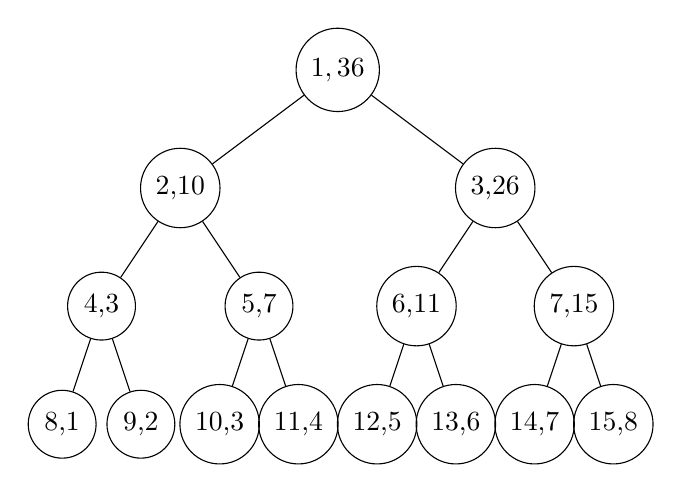
\begin{tikzpicture}[level distance=1.5cm,
  level 1/.style={sibling distance=4cm},
  level 2/.style={sibling distance=2cm},
  level 3/.style={sibling distance=1cm},
  level 4/.style={sibling distance=0.5cm},]
\node[circle,draw](z){$1,36$}
	child{
		node[circle,draw]{2,10} child{
		node[circle,draw]{4,3} child {
			node[circle,draw]{8,1} 
		} child {
			node[circle,draw]{9,2} 
		} 
	} child{
		node[circle,draw]{5,7} child {
			node[circle,draw]{10,3} 
		} child {
			node[circle,draw]{11,4} 
		} 
	} 
	}
	child{
		node[circle,draw]{3,26} child{
		node[circle,draw]{6,11} child {
			node[circle,draw]{12,5} 
		} child {
			node[circle,draw]{13,6} 
		} 
	} child{
		node[circle,draw]{7,15} child {
			node[circle,draw]{14,7} 
		} child {
			node[circle,draw]{15,8} 
		} 
	} 
	}
;
\end{tikzpicture}\\
list:\\
$[$ $a_1$,$a_2$,$a_3$,$a_4$,$a_5$,$a_6$,$a_7$,$a_8$ $]$\\
\\Claim1: The number of nodes in the binary heap will always be 2n-1.\\
Prove by induction:\\
when n=1, the binary heap has only one node. Claim stands.\\
when n=k, by definition, the binary heap now have k leaves. (we can always build that kind of binary heap uniquely because of the property of binary heap) Assume that the tree now have 2k-1 nodes. From the formation of binary heap, we know that the heap does not have a node with only one node, means that every leave has its own sibling. Suppose we want to the binary tree to have k+1 leaves. we need to add one node to the binary heap. Since every leave has its own sibling, to add a node to the current tree, we need to turn one current leaf into a internal node( node that is not leave), and add two leaves to it. So, the number of nodes will be 2k-1+2=2(k+1)-1. By induction, we are done.\\
Claim2: The height of the binary heap will be at most log(n)+1.\\ From Claim1 we know that the heap contains 2n-1 nodes, so from the property of binary heap we know that the height of binary heap will be at most log(m), where m is the number of nodes. So, the height of such heap with n leaves will be at most log(2n-1), which is at most log(n)+1.\\
Claim3:The leaf has coordinate (n+i-1,$a_i$)\\
From claim1 whe know that there are 2n-1 nodes, so the key of the first leaf is: (2n-1) - n + 1 ( the number of not-leaf-nodes plus one). The same works for other leaves.\\
b.\\
First, Init. \\
To initialize a binary heap with m nodes, the time complicity is O(m), so to initialize a binary heap with n leaves, which means it has 2n-1 nodes, we first create a binary heap with 0 in every node and a key in the order of the creation of the node, which takes 2n-1 steps. Then, we create a list stores the pointer to those nodes $a_i$: (the nodes created in last n steps) for each i in a list with the same length (E.g. the location for $a_1$ in that list is 0x001, the memory for $a_2$ is 0x005, the memory for $a_3$ is 0x009 etc. ), which will take n steps.(we do this to make sure extract $a_i$ will cost  O(1) ) So, the worst case running time is O(3n-1) = O(n). So, Init runs in time O(n).\\
Second, Add.\\
the pseudo code is as follow:(its in python, and has a helper
function called ADD\_on\_node):
\begin{lstlisting}
def ADD_on_node(curr_node, t):
	#this function add value to the current node
	curr_node.value = curr_node.value + t #set value
	if curr_node.isRoot() is True: #if current node is
	 root, terminate the whole operation.
		return None
	curr_node = curr_node.parent # set current node 
	to its parent
	ADD_on_node(curr_node, t) # do this thing recursively
	 along the tree's path

def ADD(self,i,t):
	curr_node = self.list[i] #extract $a_i$, take O(1)
	ADD_on_node(curr_node, t)
\end{lstlisting}

this function runs every non-recursion step in O(1) time, and it can only recursively run h time (h is the height of the tree, which is smaller than $log_2(2n-1)$), because a leaf can only have that many parents. So, the running time is O(log(n)).\\
Third, Sum.\\
the pseudo code is as follow:(its in python, and has two helper
function called is\_left, SUM\_on\_node):\\
\begin{lstlisting}
def is_right(node):
	return node.parent.key == 2 * (node.key) + 1
	# the node is a right child of its parent node if 
	and only if the key of it satisfy this condition
	from the property of a binary heap.
	# of course the root is not a right child of 
	any node.
def SUM(self,i):
	#initialize the solution to 0
	curr_node = self.list[i]
	#extract $a_i$, take O(1)
	solu = curr_node.value
	#initial the value of solution to $a_i$'s value
	if curr_node.isRoot():
		return solu
	#if current node is root, return current 
	summation and terminate the whole operation.
	else:
		solu = solu + SUM_on_node(curr_node.parent
		, solu):
	#do the recursion step
def SUM_on_node(curr_node, solu):
	if curr_node.isRoot() is True: 
	#if current node is root, return current 
	summation and terminate the whole operation.
		return solu
	elif curr_node.is_right is True:
		return SUM_on_node(curr_node.parent,
		 solu + current.parent.left.value)
	#if current node is a right child, add its 
	left sibling's value and recursively operate
	 upper to its parent.
	elif curr_node.is_right is False:
		return SUM_on_node(curr_node.parent, solu)
	#if current node is a left child, do nothing
	 add continue the recursion step.
\end{lstlisting}
this function is correct because every time operate follow the path and the current node is a right node, the summation of all left-hand-side $a_i$ of current node which we don't want to miss is stored in its left sibling. 
this function runs every non-recursion step in O(1) time, and it can only recursively run h time (h is the height of the tree, which is smaller than $log_2(2n-1)$), because a leaf can only have that many parents. So, the running time is O(log(n)).\\
c.\\
for each n = $2^k$, the number of nodes is 2n-1 = $2^{k+1}$ - 1, and the height of which is exactly $log_2(2^{k+1} - 1 +1 ) - 1$ = k. And, the recursive steps, proceed from leaf to root, is exactly h + 1 = k + 1 steps from the definition of height. Any other steps in that algorithm runs in O(1), so, the whole algorithm must run in exactly $\Omega(h + 1) = \Omega(k) = \Omega(log(n))$ steps.

\section{Question 1.}
Claim1: For a R-heap, r.d = r.left.d + 1(r is the root), and if r.left is empty, we assume it as 0.\\
Proof: when r has at most 1 child, r.d =1. r has no left child, so the claim is correct.
when r has 2 child, r.d = 1 + min (r.left.d,r.right.d), and r.left.d $\leq$ r.right.d. So, r.d = r.left.d + 1, claim is correct.
a.\\
the pseudo code is as follow:(its in C(in which we can use pointer easily), and has a helper
function called Insert):\\
precondition: H1 and H2 are not empty, and are all R-heap. 
\begin{lstlisting}
#include <*>
void Insert(R_HEAP *H1, R_HEAP *H2);
/*
  Insert a R_Heap 
*/

R_HEAP* Union (R_HEAP *H1, R_HEAP *H2){
	// its a function union 2 R_HEAPs, and returns the 
	// R_HEAP with the key in the root is equal to the 
	// smaller one of (H1, H2).
	// the two parameters are 2 pointers that pointed at 
	// the root of H1 and H2, and returns also a pointer to 
	// the root of the tree.
	
	/* the following checks if one of (H1,H2) is null.	
	if (*H1 == null):
	{
		return H2;
	}
	else if (*H2 == null):
	{
		return H1;
	}
	
	if (*H1.key > *H2.key)
		// we will always insert the tree with more key
		// value (in the root) into the one with less key
		// value in order to preserve the Min Heap Order
		// property
	{
		Insert(H2, H1);
		// do (recursively) 
		*H2.d = 1+min(*H2.left.d, *H2.right.d);
		// after correctly inserted H1 into H2, we need 
		// to undate the value of d stored in the root of H2
		// return H2;
	}
	else if (*H1.key <= *H2.key)
	{
		Insert(H1, H2);
		*H1.d = 1+min(*H2.left.d, *H2.right.d);
		return H1;
	}
}

void Insert(R_HEAP *H1, R_HEAP *H2) {
	// inserts a R_HEAP into anther. Here we assume that 
	// the key of H1 (in its root) is less than or equal to 
	// the Key of H2
	/*
		the logic here is : f the right node is null, we
		 insert H2 here.If the right node of H1 is not 
		 null, we recursively union the left child and H2.
	*/
	if (*H1.right == null)
	{
		*H1.right = *H2;
	}
	
	else if (*H1 != null)
	{
		*H1.left = Union(*H1.left, *H2);
		if (*H1.left.d > *H1.right.d)
			// here, we do a swap to preserve the 
			// R-balance property.
		{
			R_HEAP * temp = *H1.right;
			*H1.right = *H1.left;
			*H1.left = temp;
		}
	}
	
}

\end{lstlisting}
The algorithm is: we go along the R-heap with smaller key in its root. If it has no right child(means its a leaf), we put our another R-heap there.(then. the algorithm is definitely correct and in O(r1.d+r2.d)) If it has a right child already, we extract its left child, and union them recursively, then do a swap if needed to preserve  to preserve the R-balance property.(if it has no left child , just put H2 there and swap)\\
The claim is, our algorithm runs in O(r1.d+r2.d) time. First, all the steps runs in O(1) except the recursion step. Next, the loop invariant is, every time we union two R-heap, the returned thing is a R-heap. So, prove by induction. when r1.d =1 and r2 =1, we directly insert and swap, which is O(1) = O(r1.d+r2.d). Then, when when union H1 and H2 whose r1 or r2 not equal to 1, we unoin them, and evoke a insert function (see the code). When H1.right == null, the program terminate, so the running time is O(1), which is surely O(r1.d+r2.d). When H1.right != null, we run the sub-Union step, and assume that step takes O(H1.left + H2) steps. Then, the other steps need to terminate the program are all in O(1), because the returned thing is a R-heap, and root.left.d $\leq$ root.right.d, we will always find the path with smallest d along the left hand side of such R-heap. So, the following code will take O(H1.d - H1.left.d) time. So, the total time is: O(H1.d - H1.left.d) +O(H1.left + H2) = O(r1.d+r2.d).\\
b.\\
Proof:\\
r.d = r.left.d + 1, so the r.d is the length of the left branch of the R-heap. E.g. in the following graph,\\
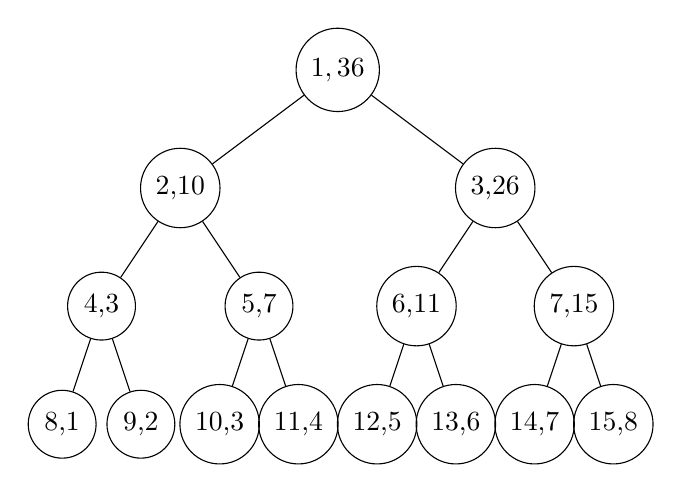
\begin{tikzpicture}[level distance=1.5cm,
  level 1/.style={sibling distance=4cm},
  level 2/.style={sibling distance=2cm},
  level 3/.style={sibling distance=1cm},
  level 4/.style={sibling distance=0.5cm},]
\node[circle,draw](z){$1,36$}
	child{
		node[circle,draw]{2,10} child{
		node[circle,draw]{4,3} child {
			node[circle,draw]{8,1} 
		} child {
			node[circle,draw]{9,2} 
		} 
	} child{
		node[circle,draw]{5,7} child {
			node[circle,draw]{10,3} 
		} child {
			node[circle,draw]{11,4} 
		} 
	} 
	}
	child{
		node[circle,draw]{3,26} child{
		node[circle,draw]{6,11} child {
			node[circle,draw]{12,5} 
		} child {
			node[circle,draw]{13,6} 
		} 
	} child{
		node[circle,draw]{7,15} child {
			node[circle,draw]{14,7} 
		} child {
			node[circle,draw]{15,8} 
		} 
	} 
	}
;
\end{tikzpicture}\\
node with key 1,2,4,8 is the most-left branch, and the length of the most-left branch is 4.\\
To prove 2.c is the same as to prove that, with the most-left branch's length is m, a R-heap has at least $2^m$-1 nodes( [r.d = m implies number of nodes $\leq$ $2^m$-1] implies [if number of nodes is n, r.d $\leq$ $log_2 (n+1)$] ).
Prove by induction:\\
base case: when the length of the most-left branch is 1, the number of nodes is at most 2, because the root won't have a left child then. The claim is correct.\\
induction hypothesis: with the most-left branch's length is k, a R-heap has at least $2^k$-1 nodes\\
when the length of the most-left branch is k+1, we just imaging create a node with no child, and append the whole R-heap with most-left branch's length is k to it. then, in order to make the tree with the length of the most-left branch is k+1 a R-heap, the right child of whose root must have d $\leq$ k, and from induction hypothesis, such right child must have at least $2^k$-1 nodes. So, the total number of that R-heap is : $2^k$-1 + $2^k$-1 + 1 = $2^{k+1}$-1. We are done.
\\c.\\
First, the height $\leq$ n, from the definition of height.
\end{document}

